\documentclass[aspectratio=169]{beamer}
%\usetheme{boxes}
\usetheme{metropolis}
\usefonttheme{professionalfonts,structurebold}
\usecolortheme{dove}

\usepackage[advantage,asymptotics,adversary,sets,keys,ff,lambda,primitives,events,operators,probability,logic,mm,complexity]{cryptocode}
\usepackage[capitalise]{cleveref}

\usepackage{scrextend} \changefontsizes{9pt}

\usepackage{paralist}

\usepackage{tikz}
\usetikzlibrary{positioning,arrows}

\title{Non malleability of the Fiat-Shamir transformation}
\author{\normalsize{Markulf Kohlweiss \inst{1} \and Michal Zajac \inst{2}}}
\institute{\inst{1}IOHK \inst{2} Clearmatics }
\date{}

\newcommand{\newdefs}[1] {\setlength{\fboxsep}{1pt}\colorbox{gray!20}{\(#1\)}}

\newcommand{\COMMENT}[1]  {}

%general formatting
\newcommand{\pcvarstyle}[1]{\mathsf{#1}}
\newcommand{\comment}[1]{{\color{lightgray}#1}}
\newcommand{\continue}{{\Huge{\hl{$\cdots$}}}}

% General mathematics
\newcommand{\range}[2] {[#1 \, .. \, #2]}
\newcommand{\SD}{\Delta}
\newcommand{\smallset}[1] {\{#1\}}
\newcommand{\bigset}[1] {\left\{#1\right\}}
\newcommand{\GRP} {\mathbb{G}}
\newcommand{\pair} {\hat{e}}
\newcommand{\brak}[1] {\left(#1\right)}
\newcommand{\sbrak}[1] {(#1)}
\newcommand{\alg}[1] {\pcalgostyle{#1}}
\newcommand{\image} {\operatorname{im}}
\newcommand{\myland} {\,\land\,}
\newcommand{\mylor} {\,\lor\,}
\newcommand{\vect}[1] {\operatorname{vect}(#1)}
\newcommand{\w}{\omega}
\newcommand{\const}{\pcpolynomialstyle{const}}
\newcommand{\p}[1]{\pcpolynomialstyle{#1}}
\newcommand{\ev}[1]{\tilde{\pcpolynomialstyle{#1}}}
\newcommand{\numberofconstrains}{\pcvarstyle{n}}
\newcommand{\expected}[1]{\mathbb{E}\left[#1\right]}
\newcommand{\infrac}[2]{#1 / #2}

% bilinear maps

\newcommand{\bmap}[2] {\left[#1\right]_{#2}}
\newcommand{\gone}[1] {\bmap{#1}{1}}
\newcommand{\gtwo}[1] {\bmap{#1}{2}}
\newcommand{\gi} {\iota}
\newcommand{\gtar}[1] {\bmap{#1}{T}}
\newcommand{\grpgi}[1] {\bmap{#1}{\gi}}


% zero knowledge
\newcommand{\oracleo}{\mathsf{O}}
\newcommand{\crs}{\pcvarstyle{crs}}
\newcommand{\td}{\pcvarstyle{td}}
\newcommand{\ip}[2]{\left\langle #1, #2\right\rangle}
\newcommand{\zkproof}{\pi}
\newcommand{\proofsystem}{\mathrm{\Psi}}
\newcommand{\ps}{\proofsystem}
\newcommand{\nuppt}{\pcmachinemodelstyle{NUPPT}}
\newcommand{\ro}{\mathcal{H}}
\newcommand{\rof}[2]{\mathbf{\Omega}_{#1, #2}}
\newcommand{\trans}{\pcvarstyle{trans}}
\newcommand{\tr}{\pcvarstyle{tr}}
\newcommand{\instsize}{\pcvarstyle{n}}
\newcommand{\KG} {\mathsf{K}}
\newcommand{\kcrs} {\KG_{\crs}}
\renewcommand{\dist}{\ddv}
\newcommand{\fs}{\pcalgostyle{FS}}
\newcommand{\sigmaprot}{\pcalgostyle{\Sigma}}
\newcommand{\se}{\pcvarstyle{se}}
\newcommand{\snd}{\pcvarstyle{snd}}
\newcommand{\zk}{\pcvarstyle{zk}}
\newcommand{\advse}{\adv_\se}

%rewinding---tree of transcripts
\newcommand{\pcboolstyle}[1]{\mathtt{#1}}
\newcommand{\treebuild}{\pcalgostyle{TreeBuild}}
\newcommand{\tree}{\pcvarstyle{tree}}
\newcommand{\counter}{\pcvarstyle{counter}}


%PLONK related
\newcommand{\plonkprot}{\mathbf{P}}
\newcommand{\plonkprotfs}{\mathbf{P}_\fs}
\newcommand{\selector}[1]{\pcvarstyle{q_{#1}}}
\newcommand{\selmulti}{\selector{M}}
\newcommand{\selleft}{\selector{L}}
\newcommand{\selright}{\selector{R}}
\newcommand{\seloutput}{\selector{O}}
\newcommand{\selconst}{\selector{C}}
\newcommand{\chz}{\mathfrak{z}}
\newcommand{\reduction}{\rdv}

\newcommand{\game}[1]{\pcalgostyle{G}_{#1}}

\newcommand{\lag}{\p{L}}
\newcommand{\pubinppoly}{\p{PI}}

% general complexity theory
% \newcommand{\RND}[1]{\pcalgostyle{RND}(#1)}
\newcommand{\RND}[1]{\pcvarstyle{R}(#1)}
\newcommand{\RELGEN}{\mathcal{R}}
\newcommand{\REL}{\mathbf{R}}
\newcommand{\LANG}{\mathcal{L}}
\newcommand{\inp}{\pcvarstyle{x}}
\newcommand{\wit}{\pcvarstyle{w}}
\newcommand{\class}[1]{\mathfrak{#1}}
\newcommand{\ig}{\pcalgostyle{IG}}
\newcommand{\accProb}{\event{acc}}
\newcommand{\frkProb}{\event{frk}}
\newcommand{\FS}{\pcalgostyle{FS}} % Fiat-Shamir transform
\newcommand{\aux}{\pcvarstyle{aux}} %auxiliary input

%Plonk and Sonic
\newcommand{\plonk}{\ensuremath{\textsc{Plonk}}}
\newcommand{\plonkmod}{\ensuremath{\plonk^\star}}
\newcommand{\plonkint}{\ensuremath{\plonk^\star}}
\newcommand{\polyprot}{\pcalgostyle{poly}}
\newcommand{\plonkintpoly}{\plonkint_\polyprot}
\newcommand{\sonic}{\textsc{Sonic}}
\newcommand{\maxdegree}{\pcvarstyle{N}}

\newcommand{\dlog}{\pcvarstyle{dlog}}

\newcommand{\ur}[1]{{#1\text{-}\mathsf{ur}}}

%forking
\newcommand{\forking}{\pcalgostyle{F}}
\newcommand{\genforking}{\pcalgostyle{GF}}

%colors
\definecolor{darkmagenta}{rgb}{0.5,0,0.5}
\definecolor{lightmagenta}{rgb}{1,0.85,1}
\definecolor{lightmagenta}{rgb}{0.9,0.9,0.9}
\definecolor{darkred}{rgb}{0.7,0,0}
\definecolor{blueish}{rgb}{0.1,0.1,0.5}
\definecolor{pinkish}{rgb}{0.9,0.8,0.8}
\definecolor{darkgreen}{rgb}{0,0.6,0}
\definecolor{lightgreen}{rgb}{0.85,1,0.85}
\definecolor{skyblue}{rgb}{0.3,0.9,0.99}

%comments
\DeclareRobustCommand{\markulf}[2]  {{\color{darkmagenta}\hl{\scriptsize\textsf{Markulf #1:} #2}}}
\DeclareRobustCommand{\michals}[2]  {{\color{blueish}\sethlcolor{pinkish}\hl{\scriptsize\textsf{Michal #1:} #2}}}
\newcommand{\task}[2]{\todo[author=\textbf{Task},inline]{({\textit{#1}}) #2}}
% \newcommand{\task}[2] {\xcommenti{Task}{#1}{#2}}
% \DeclareRobustCommand{\task}[2]  {{\color{black}\sethlcolor{yellow}\hl{\textsf{TASK #1:} #2}}}

%%% Local Variables:
%%% mode: latex
%%% TeX-master: "plonkext"
%%% End:

\renewcommand{\emph}[1]{\textbf{#1}}

\newcommand{\advfs}{\adv_\fs}
\renewcommand{\myskip}{0.5\baselineskip}

% \addtobeamertemplate{navigation symbols}{}{%
%   \usebeamerfont{footline}%
%   \usebeamercolor[fg]{footline}%
%   \hspace{1em}%
%   \insertframenumber/\inserttotalframenumber }

\setbeamertemplate{section page}
{
    \begin{centering}
    \begin{beamercolorbox}[sep=12pt,center]{part title}
    \usebeamerfont{section title}\insertsection\par
    \end{beamercolorbox}
    \end{centering}
}
\AtBeginSection{\frame{\sectionpage}}

\begin{document}

\begin{frame}
\titlepage
\end{frame}

\begin{frame}
  \frametitle{Today}
  \begin{enumerate}
    \item Our result -- what we did and why it matters?
    \item A few words about $\Sigma$-protocols and Fiat--Shamir transformation
    \item Short introduction to $\plonk$
    \item How to extract witness from $\plonk$ proof? Intuitions about
      extracting and some problems we had to solve
    \item Glimpse into our main proof for simulation extractability
  \end{enumerate}
\end{frame}

\begin{frame}
  \frametitle{Our result}
  \begin{center}
   \fbox{ \begin{minipage}{10cm}
       \begin{compactitem}
       \item We show security of non-interactive versions of $\plonk$ and
         $\sonic$ (previously only interactive protocols were analysed)
       \item We show that a class (for example $\plonk$, $\sonic$) of RO-based
         NIZKs is \emph{simulation extractable}
        \end{compactitem}
        \end{minipage}
    }
  \end{center}
  \pause
  \begin{block}{Why simulation extractability matters}
    Models situation when the adversary may see other proofs before it tries to
    break knowledge soundness\\
    Proofs done in a ``stand-alone'' model don't fit well to the real world\\
    In the real world malicious provers may see multiple proofs and learn from
    them\\
    Not covered by standard soundness / knowledge soundness definition
  \end{block}
  \pause
  \begin{block}{Example}
    Two users $\adv$ and $\bdv$.

    $\adv$ knows secret $x$ what allows him to transfer money from his
    accounts. That is, a transfer is done if $\adv$ shows a zkproof of knowledge $\zkproof$
    that shows knowledge of $x$.

    Assume $\zkproof$ is randomizable. Then $\bdv$ seeing $\zkproof$ can produce
    a valid PoK $\zkproof'$ and transfer the funds as well. \emph{But $\bdv$
      doesn't know $x$}!
  \end{block}
\end{frame}

\begin{frame}
  % \frametitle{Prior our work}
  \begin{block}{Problems}
    Efficient updatable and universal zkSNARKs use random oracle and FS
    transformation\\
    Only security of an \emph{interactive} protocol is proven\\
    Security of the non-interactive version is only \emph{conjectured}\\
    Knowledge soundness of Fiat--Shamir transformed protocols rely on \emph{forking lemma}\\
    Forking lemma shown secure only for a narrow class of protocols that
    \emph{requires only a single rewinding}\\
    Not a case for any known zkSNARK
  \end{block}
  \pause
  \vspace*{-0.5cm}
  \begin{columns}[t]
    \begin{column}{0.52\linewidth}
      \begin{block}{Previous results}
        Faust et al.~(Indocrypt 2012) shown that $\Sigma$-protocols that have
        unique-response property are simulation-extractable (after Fiat--Shamir
        transformation)
        \begin{compactitem}
        \item Covers only $3$-message protocols
        \item Witness has to be extractable from $2$ transcripts
        \item Doesn't cover protocols with $\srs$
        \end{compactitem}
      \end{block}
      \pause
    \end{column}
    \begin{column}{0.4\linewidth}
      \begin{block}{Here}
        \begin{compactitem}
        \item Generalized forking lemma to work with wider class
          of protocols -- multi-round, many transcripts to extract witness
        \item We cover protocols with $\srs$
        \end{compactitem}
      \end{block}\pause
      \begin{block}{Required properties}
        \begin{compactitem}
          \item Unique response property
          \item Trapdoor-free simulatability
 %         \item $k$-simulatability
          \item Generalized general forking lemma
          \end{compactitem}
        \end{block}
    \end{column}
  \end{columns}
\end{frame}

\section*{$\Sigma$-protocols and Fiat--Shamir transformation}
\begin{frame}
  \frametitle{$\Sigma$-protocols}
  \begin{columns}
    \begin{column}{.3\linewidth}
      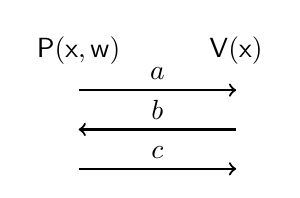
\begin{tikzpicture}
        \draw (0, 0) node (prover) {$\prover(\inp, \wit)$}; \draw (2, 0) node
        (verifier) {$\verifier(\inp)$};

        \draw[thick,->] (0, -0.5) -- node[anchor=south] {$a$} (2, -0.5);

        \draw[thick,->] (2, -1) -- node[anchor=south] {$b$} (0, -1);
        
        \draw[thick,->] (0, -1.5) -- node[anchor=south] {$c$} (2, -1.5);
      \end{tikzpicture}
    \end{column}
    \begin{column}{.6\linewidth}
      \begin{block}{Completeness}
        Honest verifier accepts proof from an honest prover.
      \end{block}
      \begin{block}{Special soundness}
        Given two transcripts for instance $(\inp, a, b, c)$ and
        $(\inp, a, b', c')$ one can compute witness $\wit$.
      \end{block}
      \begin{block}{Honest verifier zero knowledge}
        The protocol is zero-knowledge if the verifier picks its challenges randomly.
      \end{block}
      \begin{block}{Public coin}
        The verifier's challenges are public function of its randomness.
      \end{block}
    \end{column}
  \end{columns}
\end{frame}

\begin{frame}
  \frametitle{$\Sigma$-protocols. Schnorr protocol -- proof of knowledge of a discrete logarithm}
  \begin{columns}
    \begin{column}{.5\linewidth}
      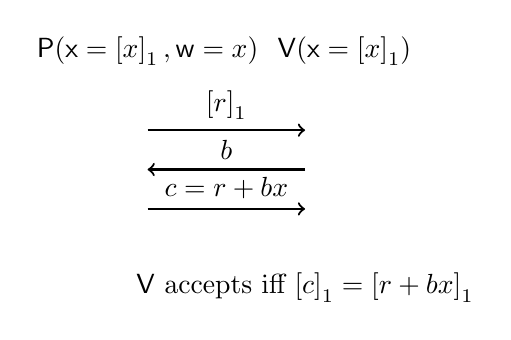
\begin{tikzpicture}
        \draw (0, 0.5) node (prover) {$\prover(\inp = \gone{x}, \wit = x)$};
        \draw (2.5, 0.5) node (verifier) {$\verifier(\inp = \gone{x})$};
        \draw[thick,->] (0, -0.5) -- node[anchor=south] {$\gone{r}$} (2, -0.5);
        \draw[thick,->] (2, -1) -- node[anchor=south] {$b$} (0, -1);
        \draw[thick,->] (0, -1.5) -- node[anchor=south] {$c = r + bx$} (2, -1.5);
        \draw (2, -2.5) node {$\verifier$ accepts iff $\gone{c} = \gone{r+ bx}$};
      \end{tikzpicture}
    \end{column}
    \begin{column}{.5\linewidth}
      \begin{block}{Special soundness}
        From $(\gone{r}, b, r + bx)$ and $(\gone{r}, b', r + b'x)$, one computes
        \[
          r + bx - (r + b'x)  = (b - b')x
        \]
        \[
          \frac{r + bx - (r + b'x)}{b - b'} = x
        \]
        Hence, for $b \neq b'$ one may reveal $x$.
      \end{block}
    \end{column}
  \end{columns}
\end{frame}

\begin{frame}
  \frametitle{$\Sigma$-protocols -- Fiat--Shamir transformation}
  \begin{columns}
    \begin{column}{.3\linewidth}
      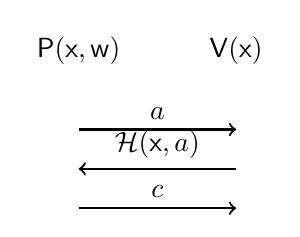
\begin{tikzpicture}
        \draw (0, 0) node (prover) {$\prover(\inp, \wit)$}; \draw (2, 0) node
        (verifier) {$\verifier(\inp)$};
        \draw[thick,->] (0, -1) -- node[anchor=south] {$a$} (2, -1);
        \draw[thick,->] (2, -1.5) -- node[anchor=south] {$\ro(\inp, a)$} (0, -1.5);
        \draw[thick,->] (0, -2) -- node[anchor=south] {$c$} (2, -2);
      \end{tikzpicture}
    \end{column}
    \begin{column}{.6\linewidth}
      \begin{block}{Completeness}
        Honest verifier accepts proof from an honest prover.
      \end{block}
      \begin{block}{Special soundness}
        Given two transcripts for instance $(\inp, a, b, c)$ and $(\inp, a, b',
        c')$ one can compute witness $\wit$.
      \end{block}
      \begin{block}{Honest verifier zero knowledge}
        The protocol is zero-knowledge if the verifier picks its challenges randomly.
      \end{block}
      \fbox{\parbox{5cm}{
      \begin{block}{Public coin}
        The verifier's challenges are public function of its randomness.
      \end{block}
    }}
    \end{column}
  \end{columns}
\end{frame}

\begin{frame}
  \frametitle{Special soundness of the Fiat--Shamir transformation}
  \begin{columns}
    \begin{column}{0.5\linewidth}
  \begin{block}{How to get two transcripts from $\advfs$}
  \begin{compactenum} 
  \item Get one transcript $(\inp, a, b = \ro(\inp, a), c)$ \pause
  \item Rewind $\advfs$ after it sent $a$ \pause
  \item Pick new $\ro$ response $b'$ for $\ro(\inp, a)$ \pause
  \item Get another transcript $(\inp, a, b', c')$
  \end{compactenum}
\end{block}\pause
  
  \begin{block}{Problem}
    $\adv$ has \emph{one shot} to convince the verifier $\verifier$.

    If $\advfs$ does not like $\verifier$'s challenge, it may pick \emph{another}
    instance $\inp$ or $a$ and try again.\\[\myskip]
    What if the adversary keeps changing the instance so we cannot get $2$
    transcripts?\\[\myskip]
  \end{block}
\end{column}\pause
\begin{column}{0.5\linewidth}
  \begin{block}{}
    What is the probability that we obtain two acceptable transcripts
    $(\inp, a, b, c)$ and $(\inp, a, b', c')$?
  \end{block}\pause
  \begin{block}{Forking lemma}
    Let $\accProb$ be a probability that $\advfs$ returns an acceptable proof.\\
    $q$ -- upper bound for a number of random oracle queries $\advfs$ may
    make.\\
    $h$ -- random oracle's range size.
    \[
      \frkProb \geq \accProb \left(\frac{\accProb}{q} - \frac{1}{h}\right).
    \]
  \end{block}
\end{column}
\end{columns}
\vspace*{0.0cm}
\centering\fbox{\parbox{10cm}{\centering What if there is more than just mere $3$
    messages?\\
    What if there is more than just mere $2$ transcripts are
  necessary?}}
\end{frame}

\section*{A short introduction to $\plonk$}
\begin{frame}[t]
  \frametitle{$\plonk$ protocol overview}
  \begin{columns}
    \begin{column}{0.6\linewidth}
  \begin{block}{}
    $n$ -- number of gates in the circuit\\
    Witness $\wit$ compounds of $3n$ elements -- left / right / output wires of
    gates\\
    Values of some wires may be public    
  \end{block}
\end{column}
\begin{column}{0.3\linewidth}
  \onslide<1,2>{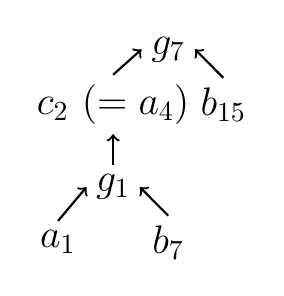
\begin{tikzpicture}[scale=0.7]
      \draw (0,0) node (gate1) {\Large{$g_1$}};
      \draw (-1, -1) node (leftinp1) {\Large{$a_1$}};
      \draw (1, -1) node (rightinp1) {\Large{$b_7$}};
      \draw (0, 1.5) node (out1) {\Large{$c_2$} $(= a_{4})$};
      \draw (1, 2.5) node (gate2) {\Large{$g_{7}$}};
      \draw (2, 1.5) node (rightinp2) {\Large{$b_{15}$}};
      \draw[thick,->] (leftinp1.north) to (gate1.west);
      \draw[thick,->] (rightinp1.north) to (gate1.east);
      \draw[thick,->] (gate1.north) to (out1.south);
      \draw[thick,->] (out1.north) to (gate2.west);
      \draw[thick,->] (rightinp2.north) to (gate2.east);
      \end{tikzpicture}}
  \end{column}
  \end{columns}
  \begin{block}{Constraint system}<2->
    \begin{compactitem}
      \item polynomials $\p{a}(X), \p{b}(X), \p{c} (X)$ with left / right /output  values at coefficients
      \item $\selleft (X), \selright (X), \seloutput (X), \ldots$ -- selector polynomials
        that tells which type the gate is.
      \end{compactitem}
    \[
      \p{a}(X) \p{b}(X) \selmulti (X) + \p{a}(X) \selleft(X) + \p{b}(X)
      \selright (X) + \p{c} (X) \seloutput (X) + \pubinppoly(X) + \selconst (X)
      = 0 \mod Z_H(X)
    \]
    for multiplication gates $\selmulti = 1, \seloutput = -1$, the rest is
    $0$\\
    for addition gates: $\selleft = 1, \selright = 1, \seloutput = -1$, the rest
    is $0$ \pause

  Additionally need to show that some relation between $\p{a} (X), \p{b} (X),
  \p{c} (X)$ holds. 
  \end{block}
\end{frame}

\begin{frame}
  \frametitle{$\plonk$ protocol overview}
  \begin{columns}[t]
    \begin{column}{0.5\linewidth}
      \textbf{Round 1.} $\prover$ encodes witness elements into $3$ polynomials:
      \begin{compactitem}
      \item \p{a'} with left input values at coefficients
      \item \p{b'} with right input values at coefficients
      \item \p{c'} with output values at coefficients
      \end{compactitem}
      Polynomials are \emph{masked} to hide coefficients even when some
      evaluations are revealed\\
      This results in polynomials $\p{a}, \p{b}, \p{c}$. \\
      Commitments $\cp{a}, \cp{b}, \cp{c}$ are computed and and sent.\pause
  \end{column}
  \begin{column}{0.5\linewidth}
    \fbox{
      \begin{minipage}{5cm}
        \begin{block}{Polynomial commitment scheme}
          $\srs = \gone{\chi, \chi^2, \ldots, \chi^d}$\\
          $\td = \chi$\\
          commitment to $\p{f}(X)$: $\gone{\p{f}(\chi)}$
        \end{block}
      \end{minipage}
    }\pause
    \end{column}
  \end{columns}
  \begin{columns}
    \begin{column}{0.5\linewidth}
    \end{column}
    \begin{column}{0.5\linewidth}
      $\verifier$ responds with challenges $\beta, \gamma$.\pause
    \end{column}
  \end{columns}
    \begin{columns}
    \begin{column}{0.5\linewidth}
      \textbf{Round 2.} $\prover$ computes \emph{permutation polynomial}
      $\p{z'}$ which is used to assure that some relation between left / right /
      output wires holds.\\
      $\p{z'}$ is masked, $\p{z}$ is created, committed and sent.
    \end{column}\pause
    \begin{column}{0.5\linewidth}
    \end{column}
  \end{columns}
      \begin{columns}
      \begin{column}{0.5\linewidth}
    \end{column}
    \begin{column}{0.5\linewidth}
      $\verifier$ responds with challenge $\alpha$.
    \end{column}
  \end{columns}

\end{frame}

  \begin{frame}[t]
    \frametitle{$\plonk$ protocol overview}
    \fbox{$\cp{a}, \cp{b}, \cp{c}, \beta, \gamma, \p{z}, \alpha$}\pause\\[\myskip]
  
  \begin{columns}
    \begin{column}{0.5\linewidth}
      \textbf{Round 3.} $\prover$ computes polynomial $t$ which is $0 \pmod
      Z_H(X)$ if all constraint equations are fulfilled, i.e.~
    \begin{compactitem}
    \item The constraint equation for the circuit, i.e.~the gates evaluate to
      correct values
    \item Permutation argument equations, i.e.~the gates that should have the
      same value, have the same value.
    \end{compactitem}
    \fbox{$\p{t}$ depends on $\p{a}, \p{b}, \p{c}, \p{z}, \alpha, \beta, \gamma$}.\\
    $\prover$ computes commitment $\p{t}$ and sends it.
  \end{column}
  \pause
  \begin{column}{0.5\linewidth}
  \end{column}
\end{columns}
\begin{columns}
  \begin{column}{0.5\linewidth}
  \end{column}
  \begin{column}{0.5\linewidth}
    $\verifier$ sends challenge $\chz$\pause
  \end{column}
\end{columns}
 \begin{columns}
    \begin{column}{0.5\linewidth}
      \textbf{Round 4.} $\prover$ evaluates polynomials $\p{a}, \p{b}, \p{c},
      \p{t}$ at $\chz$ and $\p{z}$ at $\omega \chz$.\\
      Shows correctness of the evaluation.\pause
    \end{column}
    \begin{column}{0.5\linewidth}
    \end{column}
  \end{columns}
  \begin{columns}
    \begin{column}{0.5\linewidth}
    \end{column}
    \begin{column}{0.5\linewidth}
      $\verifier$ checks that $\p{t}$ is evaluated correctly and checks other
      evaluations.
    \end{column}
  \end{columns}
\end{frame}

\section*{On extracting witness}
\begin{frame}
  \frametitle{Getting witness from $\plonk$ proof}
  Send commitments to polynomials that \alert{encode witness} $\mapsto$ Commit
  to polynomial to show that constrains are fulfilled $\mapsto$ Get \emph{opening
  challenge} $\chz$ $\mapsto$ Give \emph{evaluations} of sent polynomials at $\chz$,
  prove evaluation correctness
  \pause
  \begin{block}{The extractor}
    \begin{compactitem}
    \item Internally run $\advfs$ (knows its code)
    \item Answers $\advfs$'s random oracle queries
    \end{compactitem}
  \end{block}\pause
  \begin{block}{$\ext$:}
    \begin{compactenum}
    \item<1-> Let the adversary $\advfs$ commit to polynomials $\p{a} (X), \p{b} (X),
      \p{c} (X)$
      (only these polynomials are required to learn the whole witness)
    \item<2-> Run a proof till evaluation challenge $\chz$ is given
    \item<3-> \label{it:challenge} Pick a random $\chz$ and send it to $\advfs$
    \item<4-> Get evaluations $\p{a} (\chz), \p{b} (\chz), \p{c} (\chz)$
    \item<5-> Rewind the adversary to Step 3 and pick a new
      challenge $\chz'$ (program the random oracle)
    \item<6-> Repeat till enough evaluations are known to reveal $\p{a} (X), \p{b}
      (X), \p{c} (X)$. 
    \end{compactenum}
  \end{block}
\end{frame}

\begin{frame}
  \frametitle{Problems}
  \begin{block}{}
    \begin{enumerate}
    \item<1-> What if $\advfs$ utilizes some simulated proof up to Step
      \ref{it:challenge}?\\
      In that case we \emph{cannot rewind}
      \begin{compactitem}
      \item The adversary knows a simulated proof that starts with
        $(\inp, \cp{a}, \ldots, \cp{t})$
      \item Knows $\chz = \ro(\inp, \cp{a}, \ldots, \cp{t})$
      \item If we rewind and change $\ro$'s answer for the same
        query, $\advfs$ would notice that
      \end{compactitem}
      \fbox{Need to make sure that is not possible -- \emph{unique response
            property}}
    \item<2-> What is the probability that $\advfs$ doesn't change its mind after
      seeing new $\chz$? \\
      It could discard previously created proof and start from scratch -- pick
      new instance $\inp'$ and polynomials $\p{a'}, \p{b'}, \p{c'}$\\
      \fbox{Need a generalized version of a \emph{general forking lemma}}
    \item<3-> Standard simulation-extractability definition needs adjustment. \\
      Has to include probability $\accProb$ that adversary returns a valid proof.
    \end{enumerate}
  \end{block}
\end{frame}

\begin{frame}
  \frametitle{Problem 1 -- unique response property}
  \begin{block}{Idea}
    We say that an NI protocol has \emph{$k$-unique response property} if it is
    infeasible for a $\ppt$ adversary $\advfs$ to produce two \emph{different}
    transcripts that have the same first $k$-rounds.
  \end{block}
  \pause
  \begin{block}{}
    \begin{compactitem}
    \item $\PS$ a $(2\mu + 1)$-message protocol
    \item  Non-interactive by Fiat--Shamir
    \item $(a_1, \ldots, a_{\mu + 1})$ -- prover's messages
    \end{compactitem}

    \[
	\prob{
		\begin{aligned}
		&	\inp, \vec{a} = (a_1, \ldots, a_{\mu + 1}), \vec{a'} = (a'_1, \ldots,
    a'_{\mu + 1})
		\gets \adv^\ro(\REL, \srs), \\
    & \vec{a} \neq \vec{a'}, a_1, \ldots, a_{i} = a'_1,
    \ldots, a'_{i}, \\
		& \verifier^\ro_\fs (\REL, \srs, \inp, \vec{a}) =
		\verifier^\ro_\fs(\REL, \srs, \inp, \vec{a'}) = 1
		\end{aligned}
		\ \left|\  
	\vphantom{\begin{aligned}
	&	\vec{a} = (a_0, b_0, \ldots, a_j, b_j, a_\mu), \vec{a'} = (a'_0, b'_0, \ldots, a'_j,
	b'_j a'_\mu) \gets \adv(\REL, \srs), \vec{a} \neq \vec{a'}, \\
	& b_k = b'_k, k \in \range{1, \mu - 1},\\ a_l = a'_l, l \in
\range{1}{j}, j > i 
	\end{aligned}}
\srs \gets \kgen_\fs(\REL) \right.
} \leq \negl
\]
\end{block}

\begin{block}{Example -- Schnorr protocol}
  Transcript for instance $\gone{x}$: $(\gone{r}, b, \gone{r + bx})$\\
  After challenge $b$ is sent, $\gone{r + bx}$ is \emph{determined}
\end{block}
\end{frame}

\begin{frame}
  \frametitle{Problem 2 -- generalizing general forking lemma}
  \begin{columns}
    \begin{column}{.5\linewidth}
      \begin{block}{Tree of accepting transcript}
        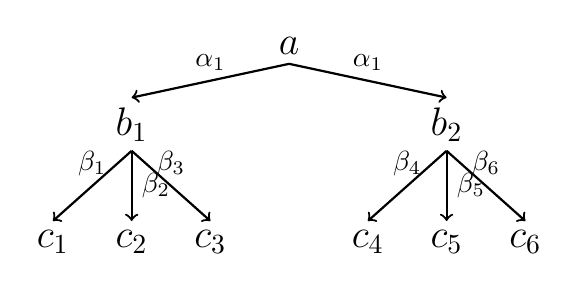
\begin{tikzpicture}
          \draw (0,0) node (a) {\Large{$a$}};

          \draw (-2, -1) node (b1)
          {\Large{$b_1$}};

          \draw (2, -1) node (b2) {\Large{$b_2$}};

          \draw (-3, -2.5) node (c1) {\Large{$c_1$}};

          \draw (-2, -2.5) node (c2)
          {\Large{$c_2$}};

          \draw (-1, -2.5) node (c3) {\Large{$c_3$}};

          \draw (1, -2.5) node (c4) {\Large{$c_4$}};

          \draw (2, -2.5) node (c5)
          {\Large{$c_5$}};

          \draw (3, -2.5) node (c6) {\Large{$c_6$}};
          
          \draw[thick,->] (a.south) to node[anchor=south] {$\alpha_1$}
          (b1.north);
          
          \draw[thick,->] (a.south) to node[anchor=south]
          {$\alpha_1$} (b2.north);
          
          \draw[thick,->] (b1.south) to
          node[anchor=south] {$\beta_1$} (c1.north);

          \draw[thick,->] (b1.south)
          to node[anchor=west] {$\beta_2$} (c2.north);

          \draw[thick,->]
          (b1.south) to node[anchor=south] {$\beta_3$} (c3.north);
          
          \draw[thick,->] (b2.south) to node[anchor=south] {$\beta_4$}
          (c4.north);

          \draw[thick,->] (b2.south) to node[anchor=west]
          {$\beta_5$} (c5.north);

          \draw[thick,->] (b2.south) to
          node[anchor=south] {$\beta_6$} (c6.north);
        \end{tikzpicture}
        Prover's messages: $a, b_i, c_j$\\
        Verifier's challenges $\alpha_k, \beta_l$\\[\myskip]
        We call such a tree a \emph{$(2, 3)$-tree of acceptable transcripts}\\[\myskip]
        Used to generalize \emph{special soundness}
        $(2,3)$-special sound protocol -- i.e.~we can get a witness from a tree
        of \emph{acceptable} transcripts as above
      \end{block}\pause
    \end{column}
    \begin{column}{.5\linewidth}
      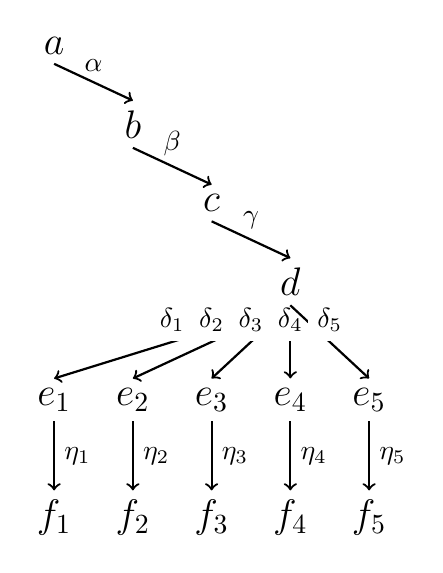
\begin{tikzpicture}
        \draw (0,0) node (a) {\Large{$a$}};

        \draw (1, -1) node (b) {\Large{$b$}};

        \draw (2, -2) node (c) {\Large{$c$}};

        \draw (3, -3) node (d) {\Large{$d$}};

        \draw (0, -4.5) node (e1) {\Large{$e_1$}};

        \draw (1, -4.5) node (e2) {\Large{$e_2$}};

        \draw (2, -4.5) node (e3) {\Large{$e_3$}};

        \draw (3, -4.5) node (e4) {\Large{$e_4$}};

        \draw (4, -4.5) node (e5) {\Large{$e_5$}};
        
        \draw (0, -6) node (f1) {\Large{$f_1$}};

        \draw (1, -6) node (f2) {\Large{$f_2$}};

        \draw (2, -6) node (f3) {\Large{$f_3$}};

        \draw (3, -6) node (f4) {\Large{$f_4$}};

        \draw (4, -6) node (f5) {\Large{$f_5$}};
        
        \draw[thick,->] (a.south) to node[anchor=south] {$\alpha$} (b.north);

        \draw[thick,->] (b.south) to node[anchor=south] {$\beta$} (c.north);

        \draw[thick,->] (c.south) to node[anchor=south] {$\gamma$} (d.north);

        \draw[thick,->] (d.south) to node[fill=white,anchor=south] {$\delta_1$}
        (e1.north);

        \draw[thick,->] (d.south) to node[fill=white,anchor=south] {$\delta_2$}
        (e2.north);

        \draw[thick,->] (d.south) to
        node[fill=white,anchor=south] {$\delta_3$} (e3.north);

        \draw[thick,->] (d.south) to node[fill=white,anchor=south] {$\delta_4$}
        (e4.north);

        \draw[thick,->] (d.south) to node[fill=white,anchor=south] {$\delta_5$}
        (e5.north);

        \draw[thick,->] (e1.south) to node[anchor=west] {$\eta_1$} (f1.north);

        \draw[thick,->] (e2.south) to node[anchor=west] {$\eta_2$} (f2.north);

        \draw[thick,->] (e3.south) to node[anchor=west] {$\eta_3$} (f3.north);

        \draw[thick,->] (e4.south) to node[anchor=west] {$\eta_4$} (f4.north);

        \draw[thick,->] (e5.south) to node[anchor=west] {$\eta_5$} (f5.north);
      \end{tikzpicture}
      $(1, 1, 1, 5, 1)$-tree of acceptable transcripts
    \end{column}
  \end{columns}
\end{frame}

\begin{frame}
  \frametitle{Problem 2 -- generalizing general forking lemma}
      \begin{columns}[t]
      \begin{column}{.5\linewidth}
        \begin{block}{Recall}
          Forking lemma states that probability of getting $2$ acceptable
          transcripts $(\inp, a, b, c)$, $(\inp, a, b', c')$ is at least
    \[
      \frkProb \geq \accProb \left(\frac{\accProb}{q} - \frac{1}{h}\right).
    \]
  \end{block}\pause
\end{column}
\begin{column}{0.5\linewidth}
  \begin{block}{Generalized forking lemma}
    Let $\Psi$ be a $(2\mu + 1)$-message (interactive) protocol\\
    Assume $\Psi$ is $m$-special sound\\
    Assume that the witness can be extracted from a $(1, ..., m, ..., 1)$-tree
    of acceptable transcript\\[\myskip]

    \[
      \frkProb = \frac{\accProb^m}{q^{m - 1}} - \accProb \cdot \left(1 -
        \frac{h!}{(h - m)! \cdot h^{m}}\right).
    \]
  \end{block}
\end{column}
\end{columns}
\end{frame}

\newcommand{\zkproofs}{\zkproof_\simulator}
\newcommand{\inpa}{\inp_{\adv}}
\newcommand{\zkproofa}{\zkproof_\adv}
\newcommand{\exta}{\ext_\adv}

\begin{frame}
  \frametitle{Simulation extractability definition}
  \begin{definition}[Forking simulation-extractable NIZK]
	\label{def:simext}
	Let $\ps = (\kgen, \prover, \verifier, \simulator)$ be a forking-sound HVZK
  proof and $\ps_\fs = (\kgen_\fs, \prover_\fs, \verifier_\fs, \simulator_\fs)$
  be $\ps$ transformed by the Fiat--Shamir transform. We say that $\ps_\fs$ is
  \emph{forking simulation-extractable} with \emph{extraction error} $\nu$ if
  for any $\ppt$ adversary $\adv$ that is given oracle access to a random oracle
  $\ro$ and simulator $\simulator_\fs$, and produces an accepting transcript of
  $\ps$ with probability $\accProb$
	probability
	\[
		\extProb = \Pr \left[
		\begin{aligned}
			& \verifier_\fs(\REL, \srs, \inp_{\advse}, \zkproof_{\advse}) = 1,\\
			& (\inp_{\advse}, \zkproof_{\advse}) \not\in Q,\\
			& \REL(\inp_{\advse}, \wit_{\advse}) = 1
		\end{aligned}
		\, \left| \,
		\begin{aligned}
			& \srs \gets \kgen_\fs(\REL), r \sample \RND{\advse},\\
			& (\inp_{\advse}, \zkproof_{\advse}) \gets \advse^{\simulator_\fs,
			\ro} (\REL, \srs; r) \\
			& \wit_{\advse} \gets \ext_\se (\REL, \srs, \advse, r, \inp_{\advse}, \zkproof_{\advse},
			Q, Q_\ro) 
		\end{aligned}
		\right.\right]
	\]
	is at at least 
	\[
		\extProb \geq \frac{1}{\poly} (\accProb - \nu)^d - \eps(\secpar)\,,
	\]
	for some polynomial $\poly$, constant $d$ and negligible $\eps(\secpar)$ whenever
  $\accProb \geq \nu$. List $Q$ contains all $(\inp, \zkproof)$ pairs where
  $\inp$ is an instance provided to the simulator by the adversary and
  $\zkproof$ is the simulator's answer. List $Q_\ro$ contains all $\advse$'s
  queries to $\ro$ and $\ro$'s answers.
\end{definition}

\end{frame}

\begin{frame}
  \frametitle{The main theorem}
\begin{theorem}[Forking simulation-extractable multi-message protocols]
  \label{thm:se}
  \onslide<1->{Let $\ps = (\kgen, \prover, \verifier, \simulator)$ be an interactive
  $(2 \mu + 1)$-message proof system for $\RELGEN(\secparam)$ that is
  \begin{compactitem}
  \item honest verifier zero-knowledge in the standard model, 
  \item has $\ur{k}$ property with security $\epsur(\secpar)$, and 
  \item is $(1, \ldots, n, \ldots, 1)$-forking sound.
  \end{compactitem}}
  % for
  % $n_i = 1, i \in \range{1}{\mu} \setminus \smallset{k}$ and $n_k = n$.
%
  \onslide<2->{Let $\ro\colon \bin^{*} \to \bin^{\secpar}$ be a random oracle.}

  \onslide<3->{Then $\psfs$ is forking simulation-extractable with extraction error
  $\epsur(\secpar)$ against $\ppt$ algebraic adversaries that makes up to $q$
  random oracle queries and returns an acceptable proof with probability at
  least $\accProb$.  The extraction probability $\extProb$ is at least
  \( \extProb \geq \frac{1}{q^{n - 1}} (\accProb - \epsur(\secpar))^{n}
  -\eps(\secpar)\,, \) for some negligible $\eps(\secpar)$.}
\end{theorem}
\end{frame}

\begin{frame}
  \frametitle{Proof idea}
  Game hops -- starting from simulation-extractability game.\\
  Define games and show that probability they abort is negligible\pause

\begin{block}{Game 0}
  Simulation extractability game: $\adv$ has access to $\oracles$ and eventually
  outputs $(\inpa, \zkproofa)$

  Game aborts if extractor $\ext_\adv$ fails to extract the corresponding witness
\end{block}\pause

\begin{block}{Game 1}
  The game is identical to Game 0, except it additionally aborts if the
  adversary output proof $\zkproof$ that matches at first $k$ places with some
  simulated proof, i.e.
  \[
    (\inpa, \zkproof[1..k]) = (\inpa, \zkproofs[1..k])
  \]

  If Game 1 aborts with non-negligible probability then $\adv$ may be used to
  break unique-response property od $\ps$.
\end{block}
\end{frame}

\begin{frame}
  \frametitle{Proof idea}
\begin{block}{Game 2}
  This game is identical to Game 1, except it additionally aborts if environment
  fails to build a tree of accepting transcripts $\tree$

  Probability of that event is bounded by \emph{generalized forking lemma}
\end{block}\pause

\begin{block}{Game 3}
  This game is identical to Game 2, except it additionally aborts if extractor
  $\ext_\tree$ fails to extract the witness from a tree of acceptable
  transcripts.

  From the $(1, \ldots, n, \ldots, 1)$-special soundness definition -- it is
  impossible for the adversary to make this game abort.
\end{block}

\end{frame}

\begin{frame}
  \frametitle{More on Game 1}
  \begin{columns}
    \begin{column}{0.5\linewidth}
      $\rdv(\srs)$ adversary against unique response property\\
      Internally runs $\adv^\oracles$, $\exta$\\[\myskip]

      \alert{Important} $\rdv$ doesn't know the trapdoor!\\[\myskip]

      \fbox{$\ps$ need to be simulatable without the trapdoor}\\[\myskip]

      But we can \emph{program the random oracle}
    \end{column}\pause
    \begin{column}{0.6\linewidth}
      $\rdv$ proceeds as follows
      \begin{compactitem}
      \item On $\adv$'s queries $(\inp, \wit)$ to $\oracles$, answer with
        $\simulator(\srs, \inp)$ and produce simulated proof $\zkproofs$.
      \item When $\adv$ outputs $(\inpa, \zkproofa)$ such that
          \[
            (\inpa, \zkproof[1..k]) = (\inpa, \zkproofs[1..k])
          \]
          Output proofs
          \begin{align*}
            \zkproof = &(\zkproofa[1..k], \ro(\inpa,
            \zkproofa[1..k]), \zkproofa[k + 1..\mu + 1]) \\
            \zkproof' = & (\zkproofa[1..k], \ro(\inpa, \zkproofa[1..k]),
            \zkproofs[k + 1..\mu + 1])
          \end{align*}
%          If $\zkproof = \zkproof'$ then $\adv$ didn't break simulation
%         extractability\\[\myskip] 
        \end{compactitem}
        If $\zkproof \neq \zkproof'$ then $\rdv$ breaks the unique response
        property
    \end{column}
  \end{columns}
\end{frame}
\begin{frame}
  \frametitle{How to simulate $\plonk$ without a trapdoor?}
  \begin{columns}
    \begin{column}{0.5\linewidth}
      \begin{block}{}
        \begin{compactenum}
        \item<1-> Pick polynomials $\p{a}, \p{b}, \p{c}$ randomly
        \item<2-> Pick random challenges $\beta, \gamma$
        \item<3-> Pick polynomial $\p{z}$ randomly
        \item<4-> Pick random challenge $\alpha$
        \item<5-> (!) Pick random challenge $\chz$
        \item<6-> Compute $t = \p{t}(\chz)$ (from $\p{a}, \p{b}, \p{c}, \p{z}$ and
          challenges)
        \item<7-> Pick random polynomial $\p{t'}(X)$
        \item<8-> Set $\p{\tilde{t}}(X) = \p{t'}(X) (X - \chz) + t$
        \item<9-> Compute $\p{a}(\chz), \p{b}(\chz), \ldots, \p{t}(\chz)$
        \item<10-> Compute openings of evaluations
        \end{compactenum}
      \end{block}\pause
    \end{column}
    \begin{column}{0.5\linewidth}
      {\footnotesize{
        \begin{align*}
          \p{t}(X)  = & 
                        (\p{a}(X) \p{b}(X) \selmulti(X) + \p{a}(X) \selleft(X) + 
                        \p{b}(X)\selright(X) + \\
                      & \p{c}(X)\seloutput(X) + \pubinppoly(X) +
                        \selconst(X)) 
                        \frac{1}{\p{Z_H}(X)} + \ldots
        \end{align*}
      }}

    \begin{block}{Caveat}
        An unbounded adversary $\adv$ could tell commitment to a real $\p{t}(X)$ from a
        commitment to a random $\p{\tilde{t}}(X)$.

        $\adv$ could compute $\p{t}(\chi)$ from $\p{a}(\chi),
        \p{b}(\chi), \ldots$. \pause

        \emph{Could a PPT adversary tell the difference?}
      \end{block}
    \end{column}
    \end{columns}
\end{frame}

\begin{frame}
  \frametitle{Uber assumption [Boneh, Boyen, Goh]}
  \begin{block}{Independent polynomial}
    Let $F = \smallset{f_1(X), \ldots, f_k(X)}, G = \smallset{g_1(X), \ldots, g_l(X)}$ be
    families of polynomials

    Let $h(X)$ be a polynomial such that
    \[
      a_h h(X) = \sum_{i = 1}^k a_{f, i} f_i (X) + \sum_{j = 1}^l a_{g, j} g_j
      (X) + \sum_{i, j}^{k, l} a_{f, g, i, j} f_i (X) g_j (X) 
    \]
    only iff $a_h, a_{f, i}, \ldots $ are all \emph{zero}. Then we call $h(X)$
    $(F, G)$-independent
  \end{block}\pause

  \begin{block}{Uber assumption}
    Let $F, G$ be families of polynomials and $h$ a $(F, G)$ independent
    polynomial. Let $\chi$ be a secret and random value and $r$ a random
    polynomial. Then no $\ppt$
    adversary can tell
    \begin{center}
     $\gone{f_1(\chi), \ldots, f_k(\chi)}, \gtwo{g_1, \ldots, g_l},
     \gone{r(\chi)}$ and 
     $\gone{f_1(\chi), \ldots, f_k(\chi)}, \gtwo{g_1, \ldots, g_l},
     \gone{h(\chi)}$
     \end{center}
    \end{block}
\end{frame}

\section{Questions?}

\begin{frame}
  \frametitle{Security of FS transformation---forking lemma}
  \begin{lemma}[General forking lemma]
    \label{lem:forking_lemma}
    \begin{columns}
      \begin{column}{.5\linewidth}
        Fix $q \in \ZZ$ and a set $H$ of size $h > 2$. Let $\zdv$ be a $\ppt$
        algorithm that on input $y, h_1, \ldots, h_q$ returns $(i, s)$, where
        $i \in\range{0}{q}$ and $s$ is called a \emph{side output}. Denote by
        $\ig$ a randomised instance generator. We denote by $\accProb$ the
        probability
        \[
          \condprob{i > 0}{y \gets \ig; h_1, \ldots, h_q \sample H; (i, s) \gets
            \zdv(y, h_1, \ldots, h_q)}\,.
        \]
        Let $\forking_\zdv(y)$ denote the algorithm described in
        \cref{fig:forking_lemma}, then the probability $\frkProb$ defined as
        $ \frkProb := \condprob{b = 1}{y \gets \ig; (b, s, s') \gets
          \forking_{\zdv}(y)} $ holds
        \[
          \frkProb \geq \accProb \brak{\frac{\accProb}{q} - \frac{1}{h}}\,.
        \]
      \end{column}
      \begin{column}{.4\linewidth}
	\begin{figure}
		\centering
		\fbox{
		\procedure{$\forking_\zdv (y)$}
		{
			\rho \sample \RND{\zdv}\\
			h_1, \ldots, h_q \sample H\\
			(i, s) \gets \zdv(y, h_1, \ldots, h_q; \rho)\\
			\pcif i = 0\ \pcreturn (0, \bot, \bot)\\
			h'_{i}, \ldots, h'_{q} \sample H\\
			(i', s') \gets \zdv(y, h_1, \ldots, h_{i - 1}, h'_{i}, \ldots,  h'_{q};
			\rho)\\
			\pcif (i = i') \land (h_{i} \neq h'_{i})\ \pcreturn (1, s, s')\\
			\pcind \pcelse \pcreturn (0, \bot, \bot)
		}}
		\caption{Forking algorithm $\forking_\zdv$}
		\label{fig:forking_lemma}
              \end{figure}
            \end{column}
            \end{columns}
\end{lemma}

\end{frame}


\begin{frame}
  \frametitle{Simulation-extractability of $\Sigma$-protocols}
  \begin{center}{\fbox{Let
      $\Psi_\fs$ be a Fiat--Shamir transformed $\Sigma$-protocol $\Psi$. Then
      $\Psi_\fs$ is simulation-extractable}}
\end{center}
\begin{columns}
  \begin{column}{.4\linewidth}
  \begin{block}{Caveats}
    The protocol $\Psi$ has to have \emph{unique response property}\\
    Simulation extractability depends on the probability $\accProb$
  \end{block}
\end{column}
\begin{column}{.4\linewidth}
  \begin{block}{Unique response property}
    $\Psi$ has unique response property if no $\ppt$ adversary $\adv$ can come
    up with two acceptable transcripts\\
    $(\inp, a, b, c)$ and $(\inp, a, b, c')$.
  \end{block}
\end{column}
\end{columns}
\end{frame}


\end{document}